\documentclass{sigchi}

% Use this command to override the default ACM copyright statement
% (e.g. for preprints).  Consult the conference website for the
% camera-ready copyright statement.

%% EXAMPLE BEGIN -- HOW TO OVERRIDE THE DEFAULT COPYRIGHT STRIP -- (July 22, 2013 - Paul Baumann)
% \toappear{Permission to make digital or hard copies of all or part of this work for personal or classroom use is      granted without fee provided that copies are not made or distributed for profit or commercial advantage and that copies bear this notice and the full citation on the first page. Copyrights for components of this work owned by others than ACM must be honored. Abstracting with credit is permitted. To copy otherwise, or republish, to post on servers or to redistribute to lists, requires prior specific permission and/or a fee. Request permissions from permissions@acm.org. \\
% {\emph{CHI'14}}, April 26--May 1, 2014, Toronto, Canada. \\
% Copyright \copyright~2014 ACM ISBN/14/04...\$15.00. \\
% DOI string from ACM form confirmation}
%% EXAMPLE END -- HOW TO OVERRIDE THE DEFAULT COPYRIGHT STRIP -- (July 22, 2013 - Paul Baumann)

% Arabic page numbers for submission.  Remove this line to eliminate
% page numbers for the camera ready copy 
% \pagenumbering{arabic}

% Load basic packages
\usepackage{balance}  % to better equalize the last page
\usepackage{graphics} % for EPS, load graphicx instead 
%\usepackage[T1]{fontenc}
\usepackage{txfonts}
\usepackage{times}    % comment if you want LaTeX's default font
\usepackage[pdftex]{hyperref}
% \usepackage{url}      % llt: nicely formatted URLs
\usepackage{color}
\usepackage{textcomp}
\usepackage{booktabs}
\usepackage{ccicons}
\usepackage{todonotes}

% llt: Define a global style for URLs, rather that the default one
\makeatletter
\def\url@leostyle{%
  \@ifundefined{selectfont}{\def\UrlFont{\sf}}{\def\UrlFont{\small\bf\ttfamily}}}
\makeatother
\urlstyle{leo}

% To make various LaTeX processors do the right thing with page size.
\def\pprw{8.5in}
\def\pprh{11in}
\special{papersize=\pprw,\pprh}
\setlength{\paperwidth}{\pprw}
\setlength{\paperheight}{\pprh}
\setlength{\pdfpagewidth}{\pprw}
\setlength{\pdfpageheight}{\pprh}

% Make sure hyperref comes last of your loaded packages, to give it a
% fighting chance of not being over-written, since its job is to
% redefine many LaTeX commands.
\definecolor{linkColor}{RGB}{6,125,233}
\hypersetup{%
  pdftitle={SIGCHI Conference Proceedings Format},
  pdfauthor={LaTeX},
  pdfkeywords={SIGCHI, proceedings, archival format},
  bookmarksnumbered,
  pdfstartview={FitH},
  colorlinks,
  citecolor=black,
  filecolor=black,
  linkcolor=black,
  urlcolor=linkColor,
  breaklinks=true,
}

% create a shortcut to typeset table headings
% \newcommand\tabhead[1]{\small\textbf{#1}}

\newcommand{\papertitle}{uCirKit}

% End of preamble. Here it comes the document.
\begin{document}

\title{uCirKit: a fast and easily modifiable circuit prototyping tool with printed circuit}

\numberofauthors{3}
\author{%
  \alignauthor{1st Author Name\\
    \affaddr{Affiliation}\\
    \affaddr{City, Country}\\
    \email{e-mail address}}\\
  \alignauthor{2nd Author Name\\
    \affaddr{Affiliation}\\
    \affaddr{City, Country}\\
    \email{e-mail address}}\\
  \alignauthor{3rd Author Name\\
    \affaddr{Affiliation}\\
    \affaddr{City, Country}\\
    \email{e-mail address}}\\
}

\maketitle

\begin{abstract}
% Even though considered a rapid prototyping tool, 3D printing is so slow that a reasonably sized object requires printing overnight. This slows designers down to a single iteration per day. In this paper, we propose to instead print low-fidelity wireframe previews in the early stages of the design process. Wireframe previews are 3D prints in which surfaces have been replaced with a wireframe mesh. Since wireframe previews are to scale and represent the overall shape of the 3D object, they allow users to quickly verify key aspects of their 3D design, such as the ergonomic fit.

Even though considered a prototyping tool, building a complicated circuit on a breadboard can be so slow that a fully debugged iteration requires significant time. In this paper, we propose a quick method to make prototypes in the early stages of circuit design process. Requiring no physical wires, \papertitle\ is a prototyping system in which wires and jumpers have been replaced with printed circuits and customized PCB. The results of our user study indicate a significant leap in prototyping performance using our system by X\%.

% To maximize the speed-up, we instruct 3D printers to extrude filament not layer-by-layer, but directly in 3D-space, allowing them to create the edges of the wireframe model directly one stroke at a time. This allows us to achieve speed-ups of up to a factor of 10 compared to traditional layer-based printing. We demonstrate how to achieve wireframe previews on standard FDM 3D printers, such as the PrintrBot or the Kossel mini. Users only need to install the WirePrint software, making our approach applicable to many 3D printers already in use today. Finally, wireframe previews use only a fraction of material required for a regular print, making it even more affordable to iterate.
\end{abstract}

\category{H.5.m.}{Information Interfaces and Presentation
  (e.g. HCI)}{Miscellaneous} \category{See
  \url{http://acm.org/about/class/1998/} for the full list of ACM
  classifiers. This section is required.}{}{}

\keywords{Authors' choice; of terms; separated; by semi\-colons;
  commas, within terms only; this section is required.}

\section{Introduction}
% Breadboard is currently the dominant tool in any prototyping process. Despite its popular, breadboard is not without its flaws, namely the need for jumper cables which lead to cluttered and messy prototypes.

The recent development in electric circuit rapid prototyping tools, such as ink-based electrical circuitry allows users to prototype without wiring. Unfortunately, ink-based electrical circuitry is inherently difficult to modify, because electronic components are affixed on a piece of paper or board by soldering or taping. A hard-to-modify prototyping tool slows makers down due to component reattachment to a new printed circuitry. We therefore argue that the process of how circuit rapid prototyping is used for quick modification is not yet optimal.

In order to allow makers to iterate quickly, hard-to-modify techniques, such as sketching and paper prototyping, give priority to speed over functionality. This trade-off pays off in the early phases of design because it encourages the quick exploration of several versions before committing further resources, eventually leading to a better design.

We argue that the same principle should apply to circuit prototyping – a concept we call easy-to-modify circuit prototyping. In contrast to the traditional workflow, in which the circuit prototyping is always done as time-consuming soldering or hard-to-modify ink-based techniques, easy-to-modify prototyping makes all intermediate versions as fast and easy-to-modify circuits. Only at the end, when the design is finished, the complete circuit prototype is printed as PCB (Figure 2).

One ink-based circuit prototyping approach is Inkjet — a system that prints circuits speed-up by substituting wires with conductive silver ink. Unfortunately, Inkjet requires users to attach components on the circuit with hard-to-modify approaches, such as taping or soldering.

In this paper, we present a easy-to-modify approach that not only save time, but also save the cost of components. The key idea is to combine the mechanism of breadboard and ink-based circuit printing to provide an easy-to-modify and robust approach for circuit prototyping , i.e. a 3D print in which surfaces have been replaced with a wireframe mesh. Our approach runs on both standard FDM 3D printers, such as the PrintrBot or the Kossel mini (rather than on a 5 axis robot arm [12]) and Inkjet printers (Brothers MFC) users only need to install the uCirKit software. Resin-coated photo paper helps to maximize the conductivity of the printed wires.

\section{Related Work}
The work presented in this paper builds on rapid prototyping of circuits, the simplicity of modification on circuits, multi-layer solutions, and approaches of how to assemble components on circuits.

\subsection{Conventional Circuit Prototyping Tools}
A breadboard is the most popular tool for electronic circuit prototyping due to its ease of circuit modification and its ability to build all kinds of projects including simple and complicated circuits. Even though its component-pluggable mechanism requires no soldering, complicated circuits involving IC chips built on a breadboard often result in complicated wiring when using jumpers. This significantly slows down the process of prototyping because a clutter of jumper wires overlapping each other on a breadboard and blocking the sight of a user increases difficulty in circuit modification and plugging new components.

A perfboard is also a popular prototyping tool mainly serving a purpose for component fixation resulting in a more compact and a more stable circuit. However, building a circuit on a perfboard requires soldering and connecting jumper wires that may take several hours to complete.

A printed circuit board (PCB) is usually a final stage for prototyping that provides more freedom with respect to component positioning and a much more compact circuit. However, PCBs allow no circuit modification, and it normally takes up to 2 weeks of processing time. Thus, PCBs are currently not suitable for rapid prototyping.

\subsection{Novel Designs in Circuit Prototyping}
% Advances in personal PCB fabrication devices and also material sciences have enabled new methods of prototyping.
% Recently, HCI researchers have proposed materials and also assembly methods for a variety of prototyping tools:
% Instant Inkjet Circuits \cite{Instant_Inkjet_Circuits} demonstrated the use of conductive ink to create printed, flexible circuits along with 3M conductive tape to provided a means of attaching components.
% Visible Breadboard \cite{Ochiai:2010:VED:1836845.1836950} presents the concept of a solder-less prototyping platform. LittleBits \cite{LittleBits} proposes an open-sourced library of modularized components as a means of prototyping.
% Circuit Stickers \cite{Circuit_Stickers} and Sketching in Circuit \cite{Sketching_in_Circuits} both utilize a form of conductive tape on paper as a tool.
% Lastly, LightUp \cite{LightUp} demonstrates an important concept in electronics, multi-layer circuits.

Since both breadboards and perfboards require connections via jumper wires that slow down the process of prototyping and decrease the ease of use of such tools, advances in personal PCB fabrication devices and also material sciences have enabled new methods of prototyping centering on making wire connections.
Recently, HCI researchers have proposed materials and also assembly methods for a variety of prototyping tools mainly divided into three categories based on the form of the substrate for the components: board, conductive ink and paper electronics, and modularized electronics.

\subsubsection{Board}
% Previous works in the board category features a piece of hard flat substrate for electrical components.
Visible Breadboard \cite{Visible_Breadboard} is a pluggable and jumper-wire-free prototyping platform by employing a capacitive touch layer for cable connections that averagely saves up to approximately 55\% of time compared to that of building the same circuit on a breadboard. Yet, \cite{Visible_Breadboard} is not compatible with most standardized components due to its dimensions causing inapplicability aside from elementary education.

\subsubsection{Conductive Ink and Paper Electronics}
Instant Inkjet Circuits \cite{Instant_Inkjet_Circuits} demonstrated the use of conductive ink to create printed, flexible circuits along with 3M conductive tape to provide a means of attaching components. 
% \cite{Instant_Inkjet_Circuits} using off-the-shelf conventional printers and replacing the default ink with cartridges filled with silver nano-particle ink.
Although \cite{Instant_Inkjet_Circuits} claims to be a rapid prototyping tool that replaces manual wiring, printed circuit paper (PCP) suffers from 2 major drawbacks. One is the single-layer issue that limits the routing of complicated circuits. Another is the modification issue where all of components need to be reattached to a piece of new PCP after correcting a design error on a previous piece of PCP.

Circuit Stickers \cite{Circuit_Stickers} extends the use of \cite{Instant_Inkjet_Circuits} and proposes a method to affix components using stickers to create more reliable circuits by expanding contact areas.
Sketching in Circuit \cite{Sketching_in_Circuits} utilizes copper tape on paper as a tool to replace jumper wire connections.
ShrinkyCircuits \cite{ShrinkyCircuits} uses a conductive pen and a heat-shrinking polymer substrate to create a solderless and jumper-wire-free circuit.
\cite{Sketching_in_Circuits} and \cite{ShrinkyCircuits} are new forms of circuit prototyping focusing more on education, creativity, and design instead of targeting rapid prototyping for advanced hardware design and implementation.

\subsubsection{Modularized Electronics}
% LittleBits \cite{LittleBits} proposes an open-sourced library of modularized components as a means of prototyping.
% LightUp \cite{LightUp} demonstrates an important concept in electronics, multi-layer circuits.

LittleBits \cite{LittleBits} proposes modularized components which become functional by simply snapping parts together with magnets as a means of prototyping without the need of wiring and electrical expertise.
LightUp \cite{LightUp} transforms electrical components into blocks assisting beginners to explore fundamental concepts of engineering and electronics.
Despite \cite{LittleBits} and \cite{LightUp} being rapid prototyping tools, the encapsulation of hardware details leads to impracticability under scenarios that require customized components and complicated circuits.


% \subsection{Circuit Printing Technology}
% The core of our work is circuit printing technology. In the work Instant Inkjet Circuits, the authors proposed a method in which they used off-the-shelf conventional printers and replaced the default ink with cartridges filled with silver nano-particle ink. This opens up circuit printing technology for the masses. Not only does such a work deliver rapid circuit creation, but also opens up a possibility of rapid prototyping, which we will discuss more in the next subsection.

% \subsection{Rapid Prototyping}
% Currently, a big player in the prototyping world is LittleBits. LittleBits seeks to modularize components and reduce the difficulty of prototyping with sophisticated electronics an elementary task. Such a feat is achieved by utilizing materials such as cardboard and paper and creating tiny circuit boards out of these materials. Along with the tiny circuits, magnets provide a mechanism for attaching differing components together to prototype complicated circuits. But besides LittleBits, Visible Breadboard presents a breadboard-like routing board that employs a capacitive touch layer for cable connections. An intuitive method such as capacitive touch showed immense improvement over soldering solutions. The last member of popular prototyping methods is the application of conductive tape as a means of connection, as well as fixing components in place. Both Circuit Stickers and Sketching in Circuit are proponents of this method.

% \subsection{Multi-layer Prototyping}
% Despite the various kinds of rapid prototyping tools, multi-layer circuits are a difficult task for current methods. LightUp utilizes a stacking method in which electronic components can be layered on top of each other to create multi-layer prototyping. This third dimension allows for a third direction in which circuits can expand, and also simplifies design of complicated circuits.
\section{System Implementation}

\begin{figure*}[t]
 \begin{center}
  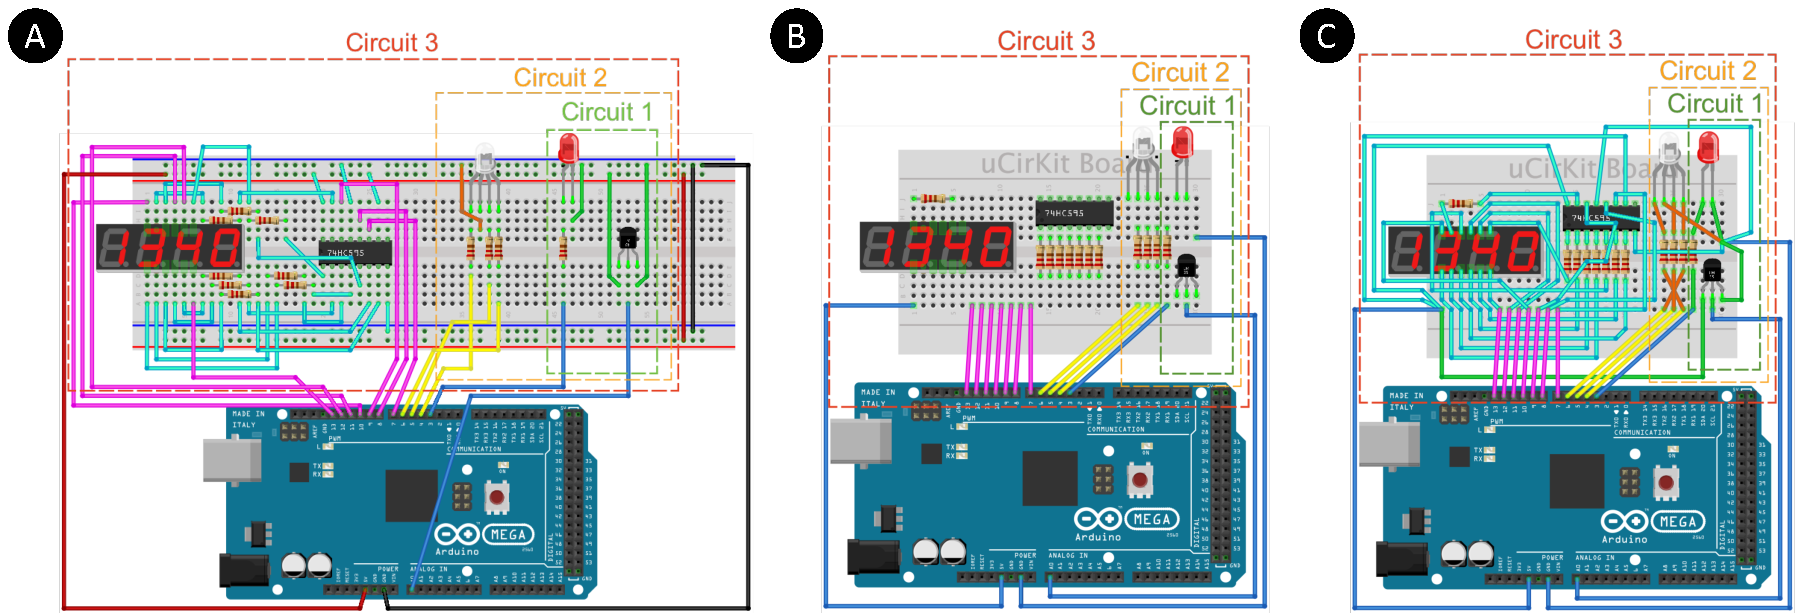
\includegraphics[width=2\columnwidth]{figures/Fritzing_Schematics_v3.pdf}
  \caption{
    Circuit 1 consists of a temperature sensor (LM35) and a LED that turns on as the temperature rises 3\textcelsius.
    Circuit 2 has a RGB LED which changes color smoothly from aqua to green to red every increment of 3\textcelsius.
    Circuit 3 is with a IC chip 74HC595 and a four-digit seven segment display  to show the temperature reading in Celsius.
    (A) and (B) are Fritzing schematics for breadboard and \papertitle, respectively. (C) shows connection arrangements hidden beneath \papertitle\ on a PCP.
  }
  \label{fig:Chosen_Circuits}
  \end{center}
\end{figure*}

% \begin{figure*}[t]
%  \begin{center}
%   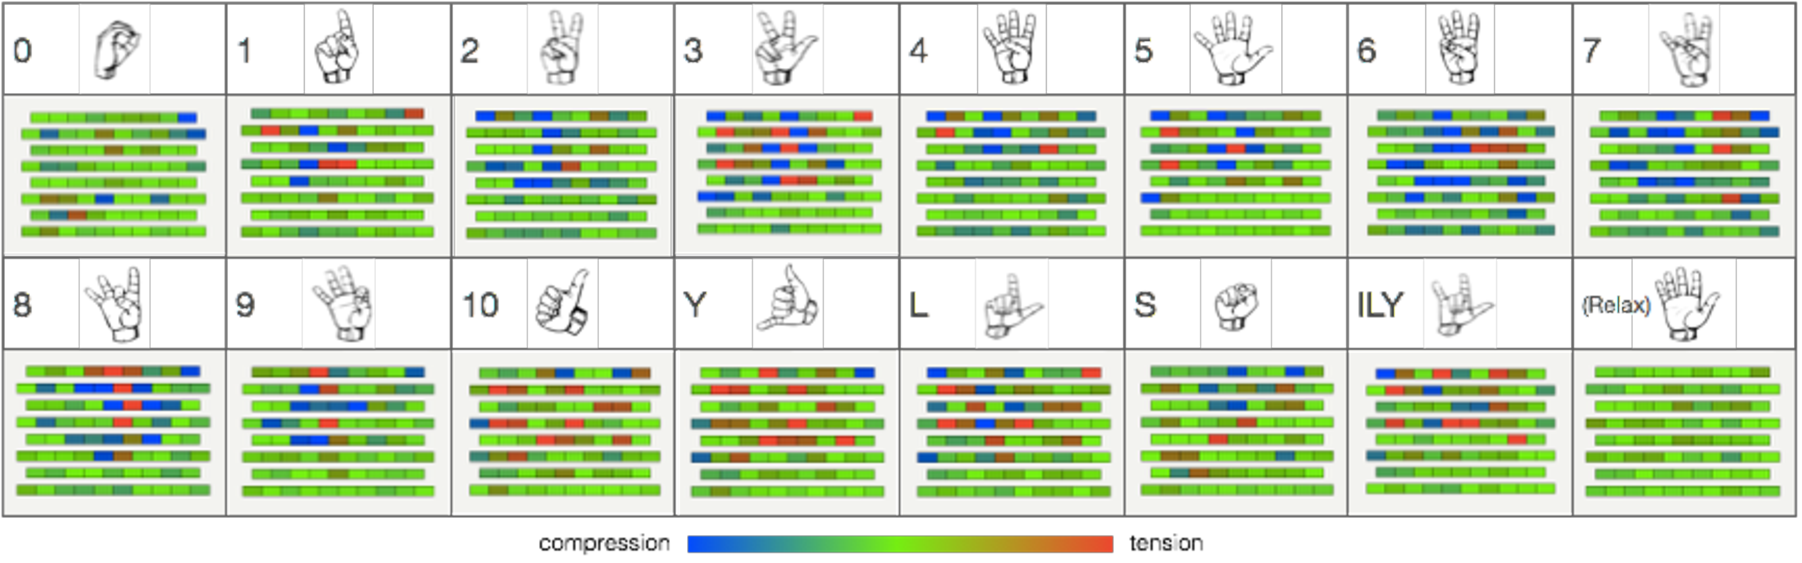
\includegraphics[width=2\columnwidth]{figures/user16GesturesSV_v3.pdf}
%   \caption{ 16 heat maps display all 16 gestures performed by one of the participants. Each entry is an average heat map of 10 trials of a gesture. The sensor reading patterns are significantly different across 16 gestures.
%   }
%   \label{fig:user16GesturesSV}
%   \end{center}
% \end{figure*}

Among the related works in the previous section, a breadboard provides easy modification by its pluggable mechanism, and PCP offers fast wiring by printing out conductive ink. Thus, we present a new rapid prototyping tool, \papertitle, simultaneously adopting a pluggable and PCP fast wiring mechanism.

\subsection{Hardware}

% Since \cite{Instant_Inkjet_Circuits} presented a successful approach to inkjet printing circuits, we adopted a similar setup with a Brother DCP-J105 printer, silver nanoparticle ink NBSIJ--MU01, resin coated paper, and transparent PET film from Mitsubishi Paper Mill.

Since \cite{Instant_Inkjet_Circuits} presented a successful approach to inkjet printing circuits, we adopted a similar setup with a Brother DCP-J105 printer and materials from Mitsubishi Paper Mill.

As illustrated in Figure X, \papertitle\ possesses a multi-layer design composed of customized PCBs. Figure X is the top layer consisting of 10-by-30 female headers resembling the appearance and the pluggable mechanism of a breadboard. Figure X indicates the bottom layers where pieces of PCP are placed. The wiring on each piece of PCP determines the connections for the component pins on the top layer. Despite showing only X layers in Figure X, \papertitle\ can stack up to even more layers to create more connections which support more complicated circuits.

Each pin and contact pad in zone A on both the top layer and the bottom layers connects to its corresponding pad on zone B. Each pad in zone B then contacts and electrically connects to its neighboring layers through a compressible on-board contact spring, part number OG-320816 (Figure X). Pads in zone A on the bottom layers are also equipped with the same contact spring to push against the conductive ink on a PCP to form reliable physical contacts. Lastly, the layers and pieces of PCP are assembled and stacked up through tightening four screws on 4 corners.

\subsection{Software}

To create wire routing on PCP for \papertitle, the Breadboard tab in Fritzing \cite{Fritzing} functions as an interface (Figure X) for users to place components and arrange connections on a custom part, \papertitle. Then, the connection information saved in a Fritzing file, extracted through a Python script, is exported to a PCB design software, EAGLE \cite{EAGLE} where final connection arrangements and autorouting for PCP are created via EAGLE user language programming (ULP) scripts.


% \begin{figure}
%   \begin{center}
%   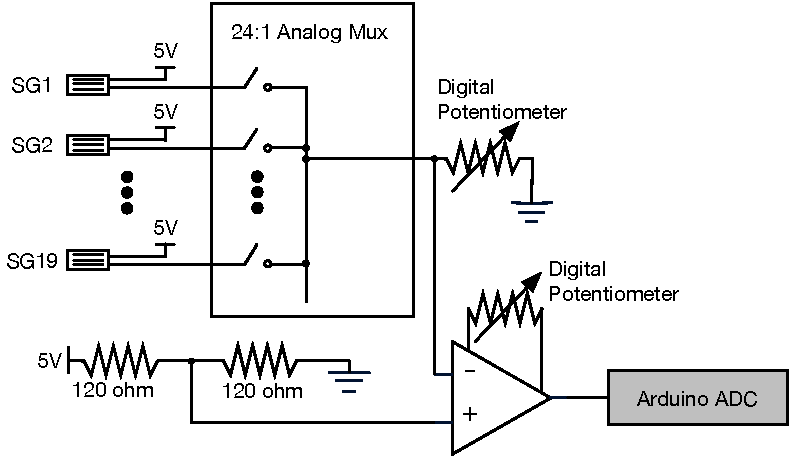
\includegraphics[width=1\columnwidth]{figures/Implementation.pdf}
%   \caption{The mechinical design of \papertitle }
%   \label{fig:FIGURE2}
%   \end{center}
% \end{figure}


% \begin{figure}
%   \begin{center}
%   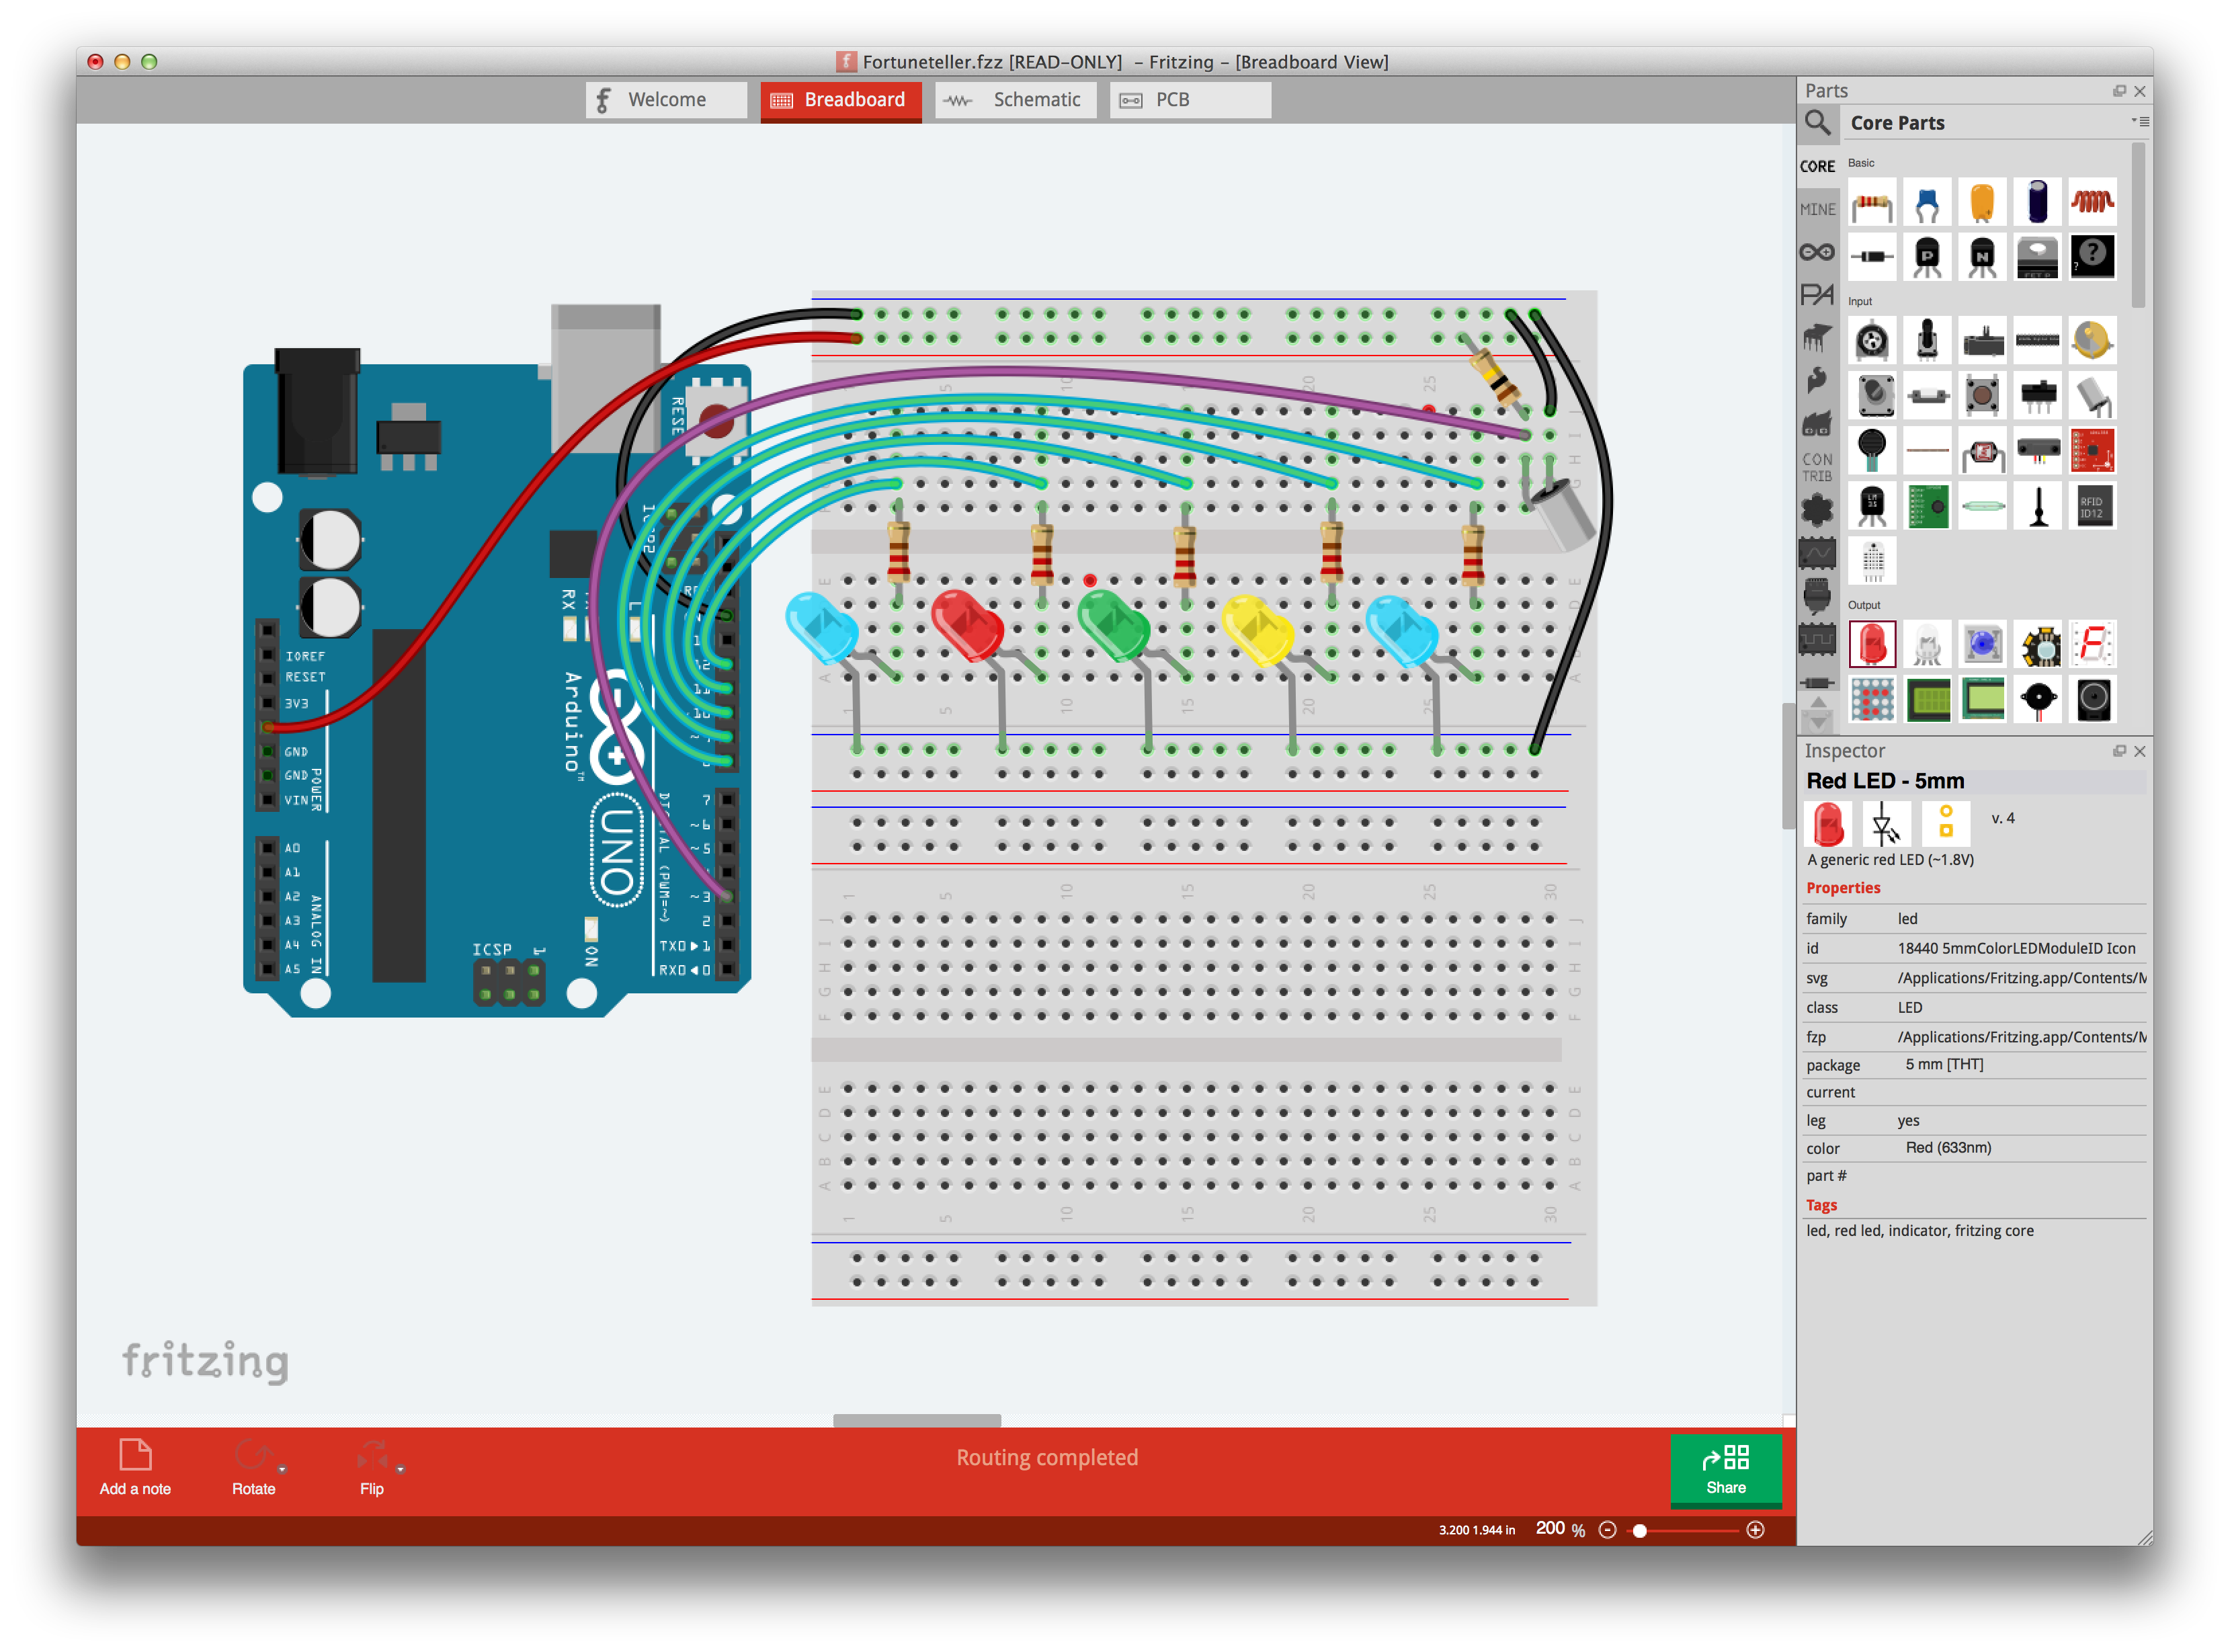
\includegraphics[width=1\columnwidth]{figures/GUI.png}
%   \caption{\papertitle also provides users a graphic user interface to help them design circuits efficiently.}
%   \label{fig:FIGURE4}
%   \end{center}
% \end{figure}
\section{User Study}

\subsection{Foreword}
The following section details the flow of our user study. However, a decision to remove printable circuits as a member of the three prototyping tools was made. This is a result of two aspects, reliability and functionality. 

The first reason was due to the unreliable nature of previous works in this area. In the beginning, we followed the convention laid out by Instant Inkjet Circuit \cite{Instant_Inkjet_Circuits}. Despite claiming to be an effective method, the 3M conductive tape suggested by Instant Inkjet Circuit proved to be a liability in component connection. Enormous pressure and heat had to be applied to obtain a consistent connection between component and printed circuit. Therefore, we modified our components to use IC sockets for an uniform 90 degree contact area. Thus, in our original study, users were given modified components in the printable circuit section.

However, the functionality of printable circuits was called into question. The high level of component customization required (e.g. Circuit Sticker) to allow for complete functionality or faster prototyping results in the lost of rapidness in prototyping. 

%In our pilot study, we found that the unreliable nature of printable circuits resulted in the lack of functionality in our implementation... Therefore...

Combining the two critical flaws mentioned above, we decided to exclude printable circuits from the tested tools in our study.

\subsection{Procedure}

\subsubsection{Pre-evaluation}
Users were first asked to answer a questionnaire in order to obtain basic information regarding age and gender. Then, users were asked how many times they have used breadboards in the past, and if they had any experience at all they were asked the source of their exposure. To help us pinpoint the users relative experience, we asked them what was the most difficult circuit they have prototyped. To conclude the pre-evaluation, users were asked they have tried other prototyping tools and if so, which ones.

\subsubsection{Environment Set-up}
Our study environment consists of three stages for each prototyping tool under evaluation. At each station, parts and Arduino Mega boards are all laid out for users to use. Users are shown schematics on a monitor in order to assist in completion of the tasks. At the same time, users are recorded in order to evaluate their process after the study is over.

\subsubsection{"Blink"}
Due to the fact that some users are completely foreign to prototyping and electronic circuits, we prepared a warm-up exercise obtained from the Official Arduino Website. The exercise, called "Blink", involves connecting a LED and turning it on and off every second by toggling the HIGH LOW of the LED. This warm-up activity was used before the start of every prototyping tool session in order to help users become acquainted with the tool they are using.

\subsubsection{Chosen Circuits}
In order to evaluate the three prototyping tools when handling circuits with different levels of complexity(?), we choose to construct a series of circuits, each building off the previous. The first circuit consists of a temperature sensor (LM35) and a LED that turns on whenever the temperature rises above 30 degrees Celsius. Without changing the first circuit, a RGB LED is then added to signify the range that the temperature is in. The RGB LED will change smoothly from aqua to green to red every increment of 3 degrees. Lastly, a four-digit seven segment is added to display the temperature reading in Celsius.

\subsubsection{Prototyping Tools}
Our evaluation encompasses breadboard, printable circuits, and lastly \papertitle\. As mentioned before, for every tool, users are asked to complete the warm-up exercise, then introduced to our chosen circuits. However, we choose to randomize the order in which users tried each tool, because REASON. Furthermore, during the chosen circuits part, some users are asked to complete the most complicated circuit, then work in reverse back to a simple LED with temperature sensor. We determined that this method would help REASON. 

\subsubsection{Post-Evaluation}
Users were recorded for the entirety of the time in which they were asked to perform the tasks above. After completion of the three tools, users were given a questionnaire that asked them to rank the convenience, ease of use, and modification ability of the three tools. Users were also given an opportunity to comment with any thoughts that they had during the study.
\section{System Evaluation}

\section{System Limitation}
Although \papertitle\ proves to be a convenient and easy to use prototyping tool, the cost for the required materials is high. For a bottle of Silver Nano Particle Ink (100 ml) the sale price is 300 USD. Additional costs of purchasing a compatible printer and customized \papertitle PCB further increase the system cost.

The printed Silver Nano Particle Ink material is not suited for extensive prototyping due to the high resistance. Therefore until there is new technology in material sciences, this material is better suited for analog circuits.

Assembly time is an area of concern due to the need for a secure and tight assembly. The use of screws and caps (FIX NAME) requires additional time to be included in the prototyping process.

\section{Future Work}
Vertical expansion -> shield form
\section{Conclusion}
In this paper, we proposed a novel approach to 3D proto- typing, i.e. to print wireframe representations instead of a filled model and to extrude filament directly into 3D space instead of printing layer-wise. Our validation shows that in combination, these two approaches indeed lead to a sub- stantial speed up of up to a factor of 10 and thus allow designers to iterate more often.

For future work, we plan to explore how fast 3D printing allows for novel types of interfaces that close the feedback loop between digital editing and physical fabrication.

% \section{Introduction}

% This format is to be used for submissions that are published in the
% conference proceedings. We wish to give this volume a consistent,
% high-quality appearance. We therefore ask that authors follow some
% simple guidelines. You should format your paper exactly like this
% document. The easiest way to do this is to replace the content with
% your own material.  This document describes how to prepare your
% submissions using \LaTeX.

% \section{Page Size and Columns}
% On each page your material should fit within a rectangle of 7 $\times$
% 9.25 inches (18 $\times$ 23.5 cm), centered on a US Letter page (8.5
% $\times$ 11 inches), beginning 0.75 inches (1.9 cm) from the top of
% the page, with a 0.33 inches (0.85 cm) space between two 3.3 inches
% (8.4 cm) columns. Right margins should be justified, not
% ragged. Please be sure your document and PDF are US letter and not A4.

% \section{Typeset Text}
% The styles contained in this document have been modified from the
% default styles to reflect ACM formatting conventions. For example,
% content paragraphs like this one are formatted using the Normal style.

% \LaTeX\ sometimes will create overfull lines that extend into columns.
% To attempt to combat this, the \texttt{.cls} file has a command,
% \texttt{{\textbackslash}sloppy}, that essentially asks \LaTeX\ to
% prefer underfull lines with extra whitespace.  For more details on
% this, and info on how to control it more finely, check out
% {\url{http://www.economics.utoronto.ca/osborne/latex/PMAKEUP.HTM}}.

% \subsection{Title and Authors}

% Your paper's title, authors and affiliations should run across the
% full width of the page in a single column 17.8 cm (7 in.) wide.  The
% title should be in Helvetica or Arial 18-point bold.  Authors' names
% should be in Times New Roman or Times Roman 12-point bold, and
% affiliations in 12-point regular.  

% See \texttt{{\textbackslash}author} section of this template for
% instructions on how to format the authors. For more than three
% authors, you may have to place some address information in a footnote,
% or in a named section at the end of your paper. Leave one 10-point
% line of white space below the last line of affiliations.

% \subsection{Abstract and Keywords}

% Every submission should begin with an abstract of about 150 words,
% followed by a set of Author Keywords and ACM Classification
% Keywords. The abstract and keywords should be placed in the left
% column of the first page under the left half of the title. The
% abstract should be a concise statement of the problem, approach, and
% conclusions of the work described. It should clearly state the paper's
% contribution to the field of HCI\@.

% \subsection{Normal or Body Text}

% Please use a 10-point Times New Roman or Times Roman font or, if this
% is unavailable, another proportional font with serifs, as close as
% possible in appearance to Times Roman 10-point. Other than Helvetica
% or Arial headings, please use sans-serif or non-proportional fonts
% only for special purposes, such as source code text.

% \subsection{First Page Copyright Notice}
% This template include a sample ACM copyright notice at the bottom of
% page 1, column 1.  Upon acceptance, you will be provided with the
% appropriate copyright statement and unique DOI string for publication.
% Accepted papers will be distributed in the conference
% publications. They will also be placed in the ACM Digital Library,
% where they will remain accessible to thousands of researchers and
% practitioners worldwide. See
% \url{http://acm.org/publications/policies/copyright_policy} for the
% ACM’s copyright and permissions policy.

% \subsection{Subsequent Pages}

% On pages beyond the first, start at the top of the page and continue
% in double-column format.  The two columns on the last page should be
% of equal length.

% \begin{figure}
% \centering
%   \includegraphics[width=0.9\columnwidth]{figures/sigchi-logo}
%   \caption{Insert a caption below each figure. Do not alter the
%     Caption style.}~\label{fig:figure1}
% \end{figure}

% \subsection{References and Citations}

% Use a numbered list of references at the end of the article, ordered
% alphabetically by last name of first author, and referenced by numbers
% in
% brackets~\cite{acm_categories,ethics,Klemmer:2002:WSC:503376.503378}.
% Your references should be published materials accessible to the
% public. Internal technical reports may be cited only if they are
% easily accessible (i.e., you provide the address for obtaining the
% report within your citation) and may be obtained by any reader for a
% nominal fee. Proprietary information may not be cited. Private
% communications should be acknowledged in the main text, not referenced
% (e.g., ``[Borriello, personal communication]'').

% References should be in ACM citation format:
% \url{http://acm.org/publications/submissions/latex_style}. This
% includes citations to internet
% resources~\cite{acm_categories,cavender:writing,CHINOSAUR:venue,psy:gangnam}
% according to ACM format, although it is often appropriate to include
% URLs directly in the text, as above.


% % Use a numbered list of references at the end of the article, ordered
% % alphabetically by first author, and referenced by numbers in
% % brackets~\cite{ethics, Klemmer:2002:WSC:503376.503378,
% %   Mather:2000:MUT, Zellweger:2001:FAO:504216.504224}. For papers from
% % conference proceedings, include the title of the paper and an
% % abbreviated name of the conference (e.g., for Interact 2003
% % proceedings, use \textit{Proc. Interact 2003}). Do not include the
% % location of the conference or the exact date; do include the page
% % numbers if available. See the examples of citations at the end of this
% % document. Within this template file, use the \texttt{References} style
% % for the text of your citation.

% % Your references should be published materials accessible to the
% % public.  Internal technical reports may be cited only if they are
% % easily accessible (i.e., you provide the address for obtaining the
% % report within your citation) and may be obtained by any reader for a
% % nominal fee.  Proprietary information may not be cited. Private
% % communications should be acknowledged in the main text, not referenced
% % (e.g., ``[Robertson, personal communication]'').

% \begin{table}
%   \centering
%   \begin{tabular}{r c c}
%     \toprule
%     & \multicolumn{2}{c}{\small{\textbf{Caption}}} \\
%     \cmidrule(r){2-3}
%     {\small\textbf{Objects}}
%     & {\small \textit{Pre-2002}}
%     & {\small \textit{Current}} \\
%     \midrule
%     Tables & Above & Below \\
%     Figures & Below & Below \\
%     \bottomrule
%   \end{tabular}
%   \caption{Table captions should be placed below the table. We
%     recommend table lines be 1 point, 25\% black. Minimize use of
%     unnecessary table lines.}~\label{tab:table1}
% \end{table}

% \section{Sections}

% The heading of a section should be in Helvetica or Arial 9-point bold,
% all in capitals. Sections should \textit{not} be numbered.

% \subsection{Subsections}

% Headings of subsections should be in Helvetica or Arial 9-point bold
% with initial letters capitalized.  For sub-sections and
% sub-subsections, a word like \emph{the} or \emph{of} is not
% capitalized unless it is the first word of the heading.

% \subsubsection{Sub-subsections}

% Headings for sub-subsections should be in Helvetica or Arial 9-point
% italic with initial letters capitalized.  Standard
% \texttt{{\textbackslash}section}, \texttt{{\textbackslash}subsection},
% and \texttt{{\textbackslash}subsubsection} commands will work fine in
% this template.

% \section{Figures/Captions}

% Place figures and tables at the top or bottom of the appropriate
% column or columns, on the same page as the relevant text (see
% Figure~\ref{fig:figure1}). A figure or table may extend across both
% columns to a maximum width of 17.78 cm (7 in.).

% \begin{figure*}
%   \centering
%   \includegraphics[width=2\columnwidth]{figures/map}
%   \caption{In this image, the map maximizes use of space. You can make
%     figures as wide as you need, up to a maximum of the full width of
%     both columns. Note that \LaTeX\ tends to render large figures on a
%     dedicated page. Image: \ccbynd~ayman on
%     Flickr.}~\label{fig:figure2}
% \end{figure*}

% Captions should be Times New Roman or Times Roman 9-point bold.  They
% should be numbered (e.g., ``Table~\ref{tab:table1}'' or
% ``Figure~\ref{fig:figure1}''), centered and placed beneath the figure
% or table.  Please note that the words ``Figure'' and ``Table'' should
% be spelled out (e.g., ``Figure'' rather than ``Fig.'') wherever they
% occur. Figures, like Figure~\ref{fig:figure2}, may span columns and
% all figures should also include alt text for improved accessibility.
% Papers and notes may use color figures, which are included in the page
% limit; the figures must be usable when printed in black-and-white in
% the proceedings.

% The paper may be accompanied by a short video figure up to five
% minutes in length. However, the paper should stand on its own without
% the video figure, as the video may not be available to everyone who
% reads the paper.  

% \subsection{Inserting Images}
% When possible, include a vector formatted graphic (i.e. PDF or EPS).
% When including bitmaps,  use an image editing tool to resize the image
% at the appropriate printing resolution (usually 300 dpi).

% \section{Language, Style and Content}

% The written and spoken language of SIGCHI is English. Spelling and
% punctuation may use any dialect of English (e.g., British, Canadian,
% US, etc.) provided this is done consis- tently. Hyphenation is
% optional. To ensure suitability for an international audience, please
% pay attention to the following:

% \begin{itemize}
% \item Write in a straightforward style.
% \item Try to avoid long or complex sentence structures.
% \item Briefly define or explain all technical terms that may be
%   unfamiliar to readers.
% \item Explain all acronyms the first time they are used in your
%   text---e.g., ``Digital Signal Processing (DSP)''.
% \item Explain local references (e.g., not everyone knows all city
%   names in a particular country).
% \item Explain ``insider'' comments. Ensure that your whole audience
%   understands any reference whose meaning you do not describe (e.g.,
%   do not assume that everyone has used a Macintosh or a particular
%   application).
% \item Explain colloquial language and puns. Understanding phrases like
%   ``red herring'' may require a local knowledge of English.  Humor and
%   irony are difficult to translate.
% \item Use unambiguous forms for culturally localized concepts, such as
%   times, dates, currencies, and numbers (e.g., ``1--5--97'' or
%   ``5/1/97'' may mean 5 January or 1 May, and ``seven o'clock'' may
%   mean 7:00 am or 19:00). For currencies, indicate equivalences:
%   ``Participants were paid {\fontfamily{txr}\selectfont \textwon}
%   25,000, or roughly US \$22.''
% \item Be careful with the use of gender-specific pronouns (he, she)
%   and other gendered words (chairman, manpower, man-months). Use
%   inclusive language that is gender-neutral (e.g., she or he, they,
%   s/he, chair, staff, staff-hours, person-years). See the
%   \textit{Guidelines for Bias-Free Writing} for further advice and
%   examples regarding gender and other personal
%   attributes~\cite{Schwartz:1995:GBF}. Be particularly aware of
%   considerations around writing about people with disabilities.
% \item If possible, use the full (extended) alphabetic character set
%   for names of persons, institutions, and places (e.g.,
%   Gr{\o}nb{\ae}k, Lafreni\'ere, S\'anchez, Nguy\~{\^{e}}n,
%   Universit{\"a}t, Wei{\ss}enbach, Z{\"u}llighoven, \r{A}rhus, etc.).
%   These characters are already included in most versions and variants
%   of Times, Helvetica, and Arial fonts.
% \end{itemize}

% \section{Accessibility}
% The Executive Council of SIGCHI has committed to making SIGCHI
% conferences more inclusive for researchers, practitioners, and
% educators with disabilities. As a part of this goal, the all authors
% are asked to work on improving the accessibility of their
% submissions. Specifically, we encourage authors to carry out the
% following five steps:
% \begin{enumerate}
% \item Add alternative text to all figures
% \item Mark table headings
% \item Add tags to the PDF
% \item Verify the default language
% \item Set the tab order to ``Use Document Structure''
% \end{enumerate}
% For more information and links to instructions and resources, please
% see: \url{http://chi2016.acm.org/accessibility}.  The
% \texttt{{\textbackslash}hyperref} package allows you to create well tagged PDF files,
% please see the preamble of this template for an example.

% \section{Page Numbering, Headers and Footers}
% Your final submission should not contain footer or header information
% at the top or bottom of each page. Specifically, your final submission
% should not include page numbers. Initial submissions may include page
% numbers, but these must be removed for camera-ready. Page numbers will
% be added to the PDF when the proceedings are assembled.

% \section{Producing and Testing PDF Files}

% We recommend that you produce a PDF version of your submission well
% before the final deadline.  Your PDF file must be ACM DL
% Compliant. The requirements for an ACM Compliant PDF are available at:
% {\url{http://www.sheridanprinting.com/typedept/ACM-distilling-settings.htm}}.

% Test your PDF file by viewing or printing it with the same software we
% will use when we receive it, Adobe Acrobat Reader Version 10. This is
% widely available at no cost. Note that most
% reviewers will use a North American/European version of Acrobat
% reader, so please check your PDF accordingly.

% When creating your PDF from Word, ensure that you generate a tagged
% PDF from improved accessibility. This can be done by using the Adobe
% PDF add-in, also called PDFMaker. Select Acrobat | Preferences from
% the ribbon and ensure that ``Enable Accessibility and Reflow with
% tagged Adobe PDF'' is selected. You can then generate a tagged PDF by
% selecting ``Create PDF'' from the Acrobat ribbon.

% \section{Conclusion}

% It is important that you write for the SIGCHI audience. Please read
% previous years’ proceedings to understand the writing style and
% conventions that successful authors have used. It is particularly
% important that you state clearly what you have done, not merely what
% you plan to do, and explain how your work is different from previously
% published work, i.e., the unique contribution that your work makes to
% the field. Please consider what the reader will learn from your
% submission, and how they will find your work useful. If you write with
% these questions in mind, your work is more likely to be successful,
% both in being accepted into the conference, and in influencing the
% work of our field.

% \section{Acknowledgments}

% Sample text: We thank all the volunteers, and all publications support
% and staff, who wrote and provided helpful comments on previous
% versions of this document. Authors 1, 2, and 3 gratefully acknowledge
% the grant from NSF (\#1234--2012--ABC). \textit{This whole paragraph is
%   just an example.}

% Balancing columns in a ref list is a bit of a pain because you
% either use a hack like flushend or balance, or manually insert
% a column break.  http://www.tex.ac.uk/cgi-bin/texfaq2html?label=balance
% multicols doesn't work because we're already in two-column mode,
% and flushend isn't awesome, so I choose balance.  See this
% for more info: http://cs.brown.edu/system/software/latex/doc/balance.pdf
%
% Note that in a perfect world balance wants to be in the first
% column of the last page.
%
% If balance doesn't work for you, you can remove that and
% hard-code a column break into the bbl file right before you
% submit:
%
% http://stackoverflow.com/questions/2149854/how-to-manually-equalize-columns-
% in-an-ieee-paper-if-using-bibtex
%
% Or, just remove \balance and give up on balancing the last page.
%
% \balance{}

% \section{References Format}
% Your references should be published materials accessible to the
% public. Internal technical reports may be cited only if they are
% easily accessible (i.e., you provide the address for obtaining the
% report within your citation) and may be obtained by any reader for a
% nominal fee. Proprietary information may not be cited. Private
% communications should be acknowledged in the main text, not referenced
% (e.g., ``[Golovchinsky, personal communication]'').

% Use a numbered list of references at the end of the article, ordered
% alphabetically by first author, and referenced by numbers in
% brackets~\cite{ethics,Klemmer:2002:WSC:503376.503378}. For papers from
% conference proceedings, include the title of the paper and an
% abbreviated name of the conference (e.g., for Interact 2003
% proceedings, use Proc.\ Interact 2003). Do not include the location of
% the conference or the exact date; do include the page numbers if
% available. See the examples of citations at the end of this document
% and in the accompanying \texttt{BibTeX} document.

% References \textit{must be the same font size as other body
%   text}. References should be in alphabetical order by last name of
% first author. Example reference formatting for individual journal
% articles~\cite{ethics}, articles in conference
% proceedings~\cite{Klemmer:2002:WSC:503376.503378},
% books~\cite{Schwartz:1995:GBF}, theses~\cite{sutherland:sketchpad},
% book chapters~\cite{winner:politics}, a journal issue~\cite{kaye:puc},
% websites~\cite{acm_categories,cavender:writing},
% tweets~\cite{CHINOSAUR:venue}, patents~\cite{heilig:sensorama}, and
% online videos~\cite{psy:gangnam} is given here. This formatting is a
% slightly abbreviated version of the format automatically generated by
% the ACM Digital Library (\url{http://dl.acm.org}) as ``ACM Ref''. More
% details of reference formatting are available at:
% \url{http://www.acm.org/publications/submissions/latex_style}.

% REFERENCES FORMAT
% References must be the same font size as other body text.
\bibliographystyle{SIGCHI-Reference-Format}
\bibliography{sample}

\end{document}

%%% Local Variables:
%%% mode: latex
%%% TeX-master: t
%%% End:
